\section{INTRODUCTION}
Modeling the thermal behavior of snow is not a new endeavor; \citet{lachapelle1960} cites a paper from 1892 that examined temperature profiles of snow. A significant amount of work has examined snow using a continuum mechanics theory of mixtures (e.g., \citet{adams1989, brown1999}.  Using a thermal non-equilibrium approach, \citet{bartelt2004} indicated that temperature differences between the pore air and ice particles and inter-facial heat exchange between snow crystals played a significant role in determining the temperature profile. Perhaps the most comprehensive model developed to date is the SNOWPACK model \citep{lehning1999, bartelt2002, lehning2002a, lehning2002b} that accounts for heat transfer, water transport, vapor diffusion, and mechanical deformation.  Research conducted in an attempt to validate the SNOWPACK model yielded reasonable results, yet \citet{fierz2001} encouraged additional work regarding the initial stage of snow metamorphism, specifically the processes involving particles changing to small faceted or rounded crystals. \citet{miller2003} and \citet{miller2009} provided a unique approach for modeling this transition. They were able to develop a model capable of faceted growth, but the model is limited in a number of ways, including an assumed spherical geometry.

Recent approaches to modeling the snowpack are based on the 3-D images of the snow micro-structure.  One notable article by \citet{kaempfer2005} utilized X-ray micro-tomography ($\mu$-CT) to build a 3-D image of a snow sample to which a finite element model was applied for modeling the heat transfer through the sample. \citet{kaempfer2009phase} demonstrated that phase-field methods may be applied to snow metamorphism and concludes that with the model ``snow metamorphism can be studied in details not possible heretofore.''

Given this broad range modeling approaches a new paradigm is needed for modeling and simulation that fosters rapid development and collaboration. The open-source Multiphysics Object Oriented Simulation Environment (MOOSE; \url{www.moooseframework.org}) is a framework specifically designed for such tasks. MOOSE is a finite-element framework that aids in application development by harnessing state-of-the-art fully-coupled, fully-implicit multiphysics solvers while providing automatic parallelization, mesh adaptivity, and an ever expanding set of physics modules including solid mechanics, phase-field, Navier-Stokes, and heat conduction. These features have provided a recipe for rapid model development (NEED REF). MOOSE natively supports multi-scale models allowing to couple MOOSE-based applications, thus fostering collaborations (NEED REF). Finally, MOOSE follows a rigorous and development strategy that ensures software quality at both the framework and application level (REF WSSSPE).

This paper briefly demonstrates the capabilities of MOOSE by:
\begin{enumerate}
\item Developing a snow micro-structure model, named Pika, based on the work \citep{kaempfer2009phase},
\item Developing a meso-scale continuum model for heat-condition, named Ibex, and
\item Coupling the two models together into a single, multi-scale simulation.
\end{enumerate}

The purpose of the work is not to provide a new model for snow, but to provided the basis for a completely new approach to modeling snow, an approach that will bring groups together to build a myriad of modeling tools that utilize a common framework.

\section{PIKA: MICRO-STRUCTURE MODEL}\label{sec:pika}
Methods and results here ...

\section{IBEX: MESO-SCALE MODEL}\label{sec:ibex}
The meso-scale model presented here is comprised of a single relationship, the heat-equation:

\begin{equation}\label{eq:meso}
\rho c_p \frac{\partial{T}}{\partial t} = \nabla \cdot k_{eff} \nabla T + s,
\end{equation}
where $T$ is temperature, $s$ a heat source term, and the material properties $\rho$, $c_p$, and $k_{eff}$ are the bulk density, specific heat, and thermal conductivity for snow. The model developed includes incoming shortwave radiation that is absorbed within the snow (i.e., the $s$ source term in Eq. \eqref{eq:meso}), including absorption that differs with wavelength as detailed by \citet[][Ch. 4]{slaughter2010numerical}. On the surface the effects of incoming and out going long-wave radiation as well as sensible and latent heat are included as detailed in \citet{morstad2007experimental}.

To demonstrate the accuracy of the model, Exp. \#2 of \citet{morstad2007experimental} was reproduced using a 1D Ibex simulation. The simulation was similar fashion as detailed in \citet[][Ch. 4]{slaughter2010numerical}. For the simulation, all input parameters were set to the value discussed in detail in \citet{slaughter2010numerical}, including incoming short- and long-wave radiation set to \unitfrac[650]{W}{m\textsuperscript{2}} and \unitfrac[235]{W}{m\textsuperscript{2}}, respectively and the albedo in the visible, near-infrared, and short-wave infrared defined as 0.94, 0.80, and 0.59, respectively.

Fig. \ref{fig:ibex_1d} includes the simulation results and a comparison with the experimental data of \citet{morstad2007experimental} after 8 hours; qualitatively the 1D Ibex model is capable capturing the general trend of experimental data. Fine tuning the parameters for Ibex is beyond the scope of this paper.

\begin{figure}[h]
  \includegraphics[width=3.125in]{figures/ibex.pdf}
  \caption{Comparison of experimental data and 1D Ibex simulation.}
  \label{fig:ibex_1d}
\end{figure}

Since, Ibex was built using MOOSE, it is dimension agnostic, thus the same code that produced the 1D results above is also capable of running in 3D with adaptive meshing, as shown in Fig. \ref{fig:ibex_3d}, without altering anything except the input file. This simulation uses the same input parameters as mentioned above, except applies the incoming short-wave irradiance as function of space and time. This demonstrates the flexibility of MOOSE-based application to build flexible and extensible applications, which will be further demonstrated in the next section.

\begin{figure}
  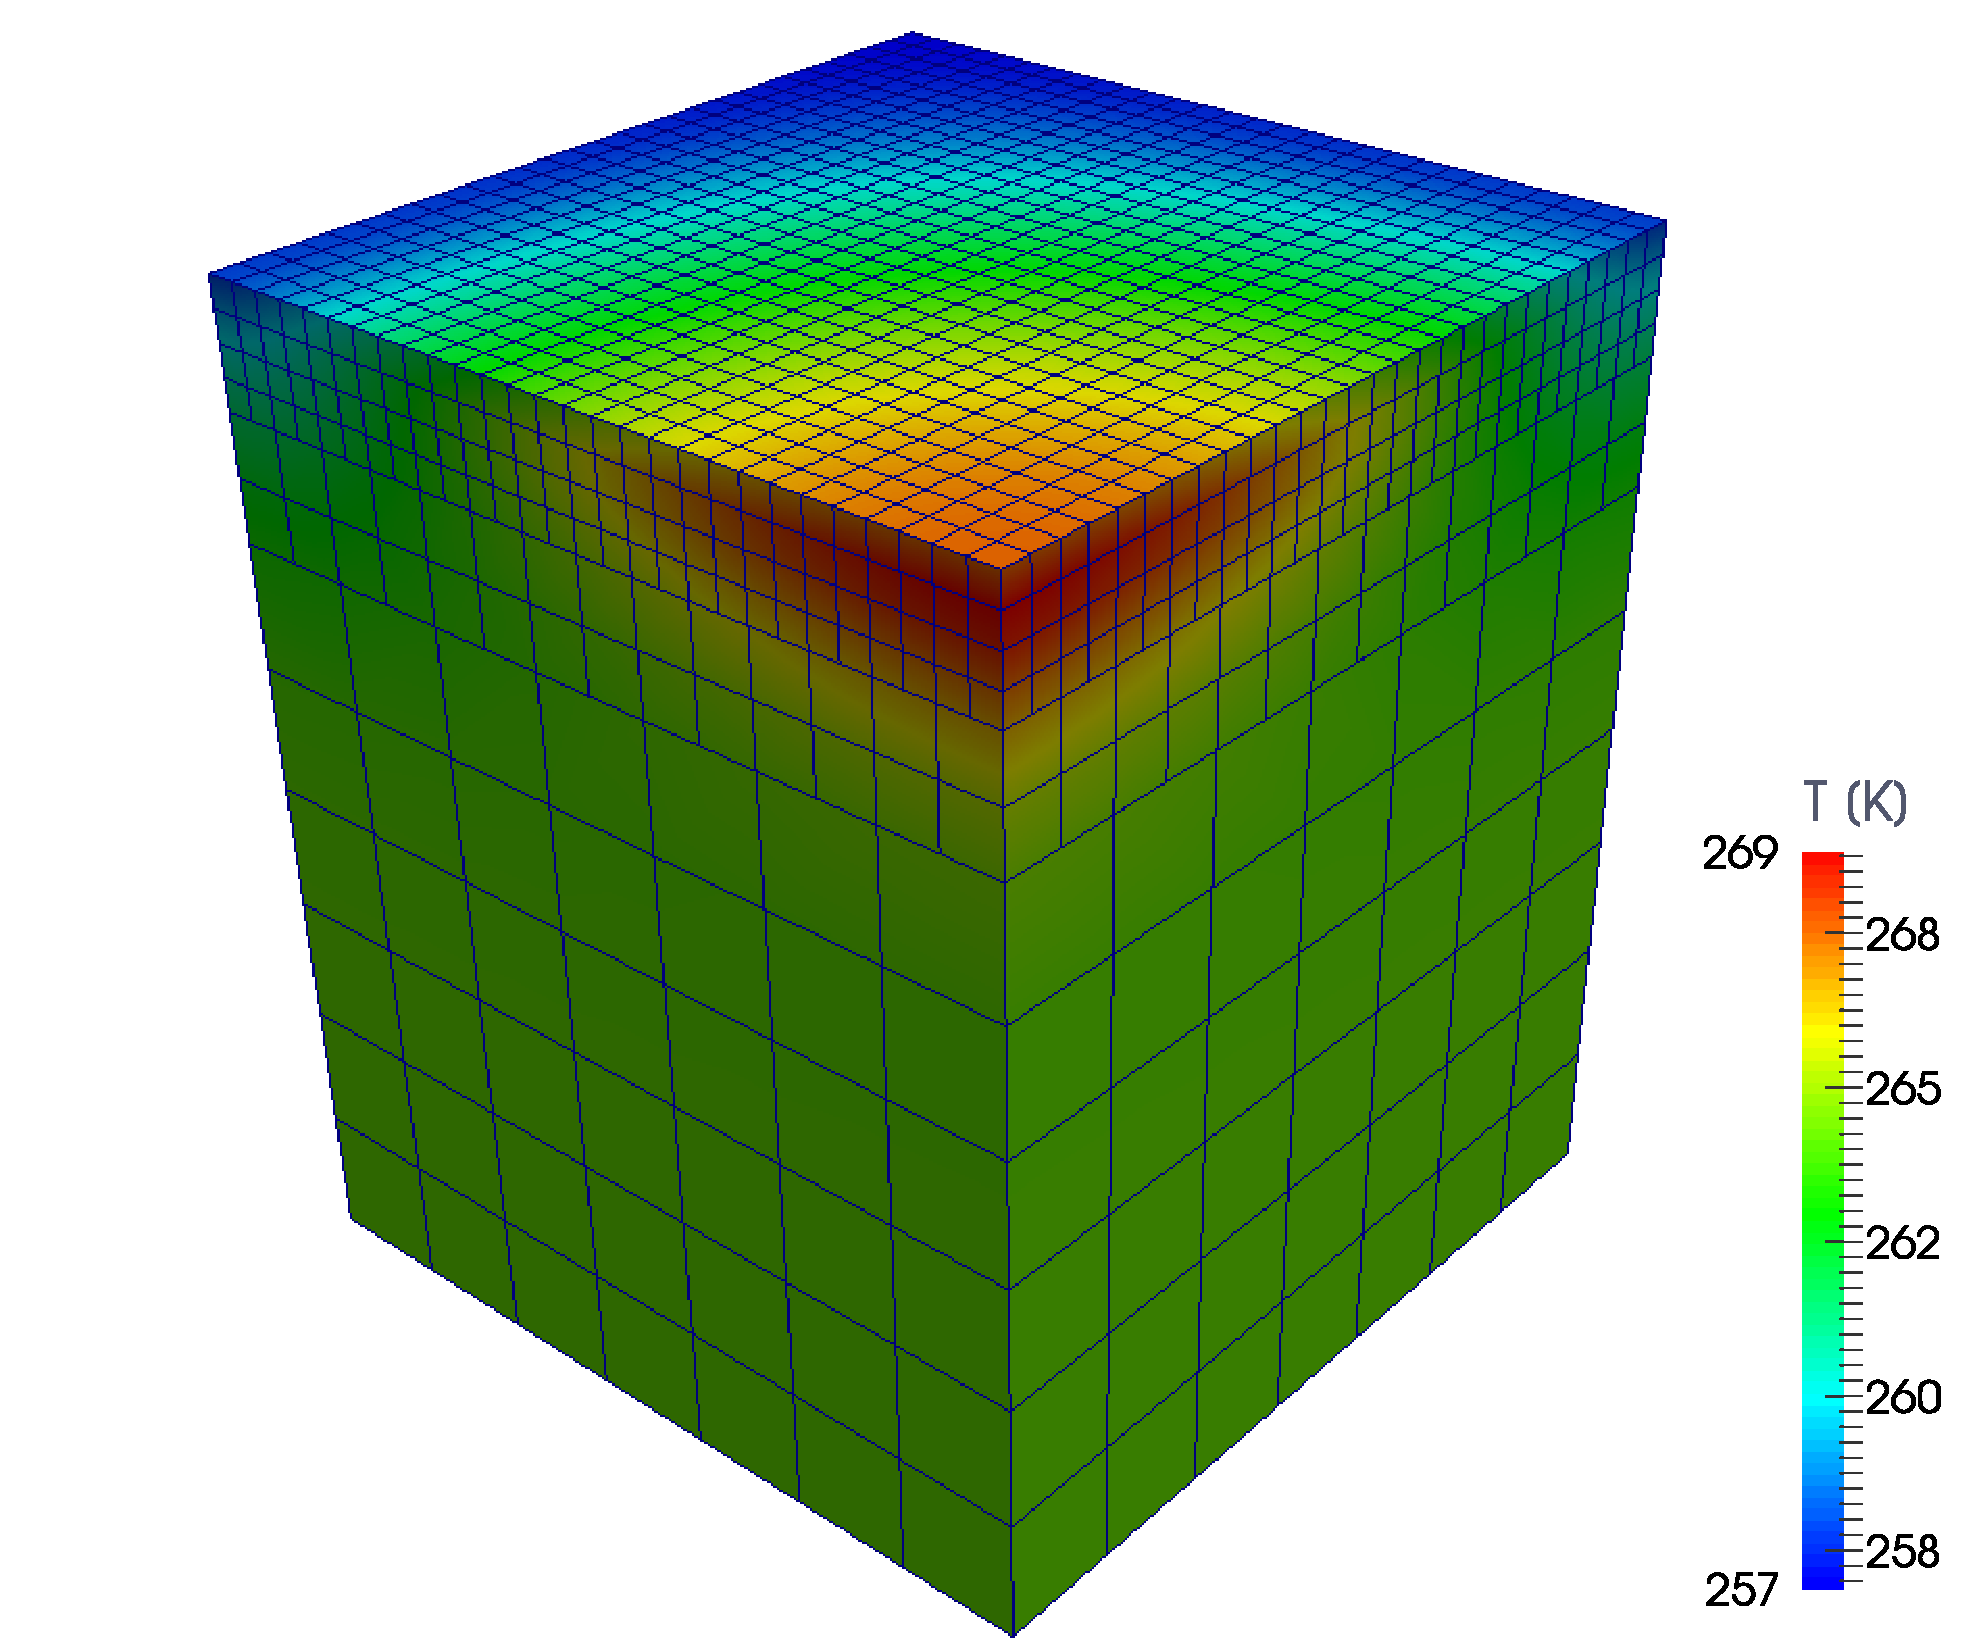
\includegraphics[width=\linewidth]{figures/ibex3d.pdf}
  \caption{Demonstration of 3D Ibex simulation with spatial and temporal varying incoming short-wave irradiance.}
  \label{fig:ibex_3d}
\end{figure}


\section{MULTI-SCALE MODEL}\label{sec:yeti}


\section{CLOSING REMARKS}
